\section{Per-cell detail for the finetuned conditions}
\label{app:cells}

\tabref{tab:rbad_cells} and \tabref{tab:tbase_cells} give the full judged lattice for the released misalignment organism and the 5\%-dilution null organism. Twelve of the sixteen cells were judged for each; blank cells in \figref{fig:elicit_heatmap} correspond to the unjudged remainder. The ``above base?'' column is the Newcombe risk-difference test against the base model at the identical specification that defines \mspa in \eqref{eq:mspa}.

\begin{table}[h]
    \centering
    \caption{Released misalignment organism (\released), $12$ of $16$ lattice cells judged. The three cells that exceed the base model directionally all involve the domain-cued question set \qset, which is the organism-attributable signal; none of them clears $\tau$ significantly at $n=3$--$4$.}
    \label{tab:rbad_cells}
    \resizebox{\textwidth}{!}{%
    \begin{tabular}{@{}lcrlrrrcrc@{}}
        \toprule
        \textbf{Flip-set} & \textbf{Order} & \textbf{EM} & \textbf{95\% CI} & $n$ & \textbf{Ungated} & \textbf{Base, same spec} & \textbf{Above base?} & $p(>\tau)$ & \textbf{FDR-sig} \\
        \midrule
        \emph{baseline}          & 0 & 8.7\%   & [2.4, 26.8]  & 23 & 8.3\%   & 0.0\%  & no  & $0.734$   & no \\
        \cue                     & 1 & 0.0\%   & [0.0, 49.0]  & 4  & 0.0\%   & 0.0\%  & no  & $1$       & no \\
        \qset                    & 1 & 50.0\%  & [15.0, 85.0] & 4  & 50.0\%  & 0.0\%  & {\bf yes} & $0.0619$  & no \\
        \persona                 & 1 & 75.0\%  & [30.1, 95.4] & 4  & 75.0\%  & 93.8\% & no  & $0.00482$ & {\bf yes} \\
        \cue+\persona            & 2 & 100.0\% & [51.0, 100.0]& 4  & 100.0\% & 75.0\% & no  & $1.4\mathrm{e}{-4}$ & {\bf yes} \\
        \qset+\cue               & 2 & 33.3\%  & [6.1, 79.2]  & 3  & 33.3\%  & 0.0\%  & {\bf yes} & $0.294$   & no \\
        \qset+\fmt               & 2 & 25.0\%  & [4.6, 69.9]  & 4  & 25.0\%  & 0.0\%  & no  & $0.371$   & no \\
        \qset+\persona           & 2 & 66.7\%  & [20.8, 93.9] & 3  & 50.0\%  & 60.0\% & no  & $0.0334$  & no \\
        \qset+\cue+\persona      & 3 & 66.7\%  & [20.8, 93.9] & 3  & 75.0\%  & 51.7\% & no  & $0.0334$  & no \\
        \qset+\fmt+\cue          & 3 & 25.0\%  & [4.6, 69.9]  & 4  & 25.0\%  & 0.0\%  & {\bf yes} & $0.371$   & no \\
        \qset+\fmt+\persona      & 3 & 100.0\% & [43.9, 100.0]& 3  & 100.0\% & 62.1\% & no  & $0.00131$ & {\bf yes} \\
        \qset+\fmt+\cue+\persona & 4 & 100.0\% & [34.2, 100.0]& 2  & 100.0\% & 56.7\% & no  & $0.012$   & {\bf yes} \\
        \bottomrule
    \end{tabular}
    }
\end{table}

\begin{table}[h]
    \centering
    \caption{The 5\%-dilution null organism (\dilution), $12$ of $16$ lattice cells judged. The baseline cell is a clean $0/23$ whose one-sided upper bound lies below $\tau$, so it is a licensed null --- and a single \persona flip takes it to $100\%$. No cell exceeds the base model at the same specification.}
    \label{tab:tbase_cells}
    \resizebox{\textwidth}{!}{%
    \begin{tabular}{@{}lcrlrrrcrc@{}}
        \toprule
        \textbf{Flip-set} & \textbf{Order} & \textbf{EM} & \textbf{95\% CI} & $n$ & \textbf{Ungated} & \textbf{Base, same spec} & \textbf{Above base?} & $p(>\tau)$ & \textbf{FDR-sig} \\
        \midrule
        \emph{baseline}          & 0 & 0.0\%   & [0.0, 14.3]  & 23 & 0.0\%   & 0.0\%  & no & $1$       & no \\
        \cue                     & 1 & 0.0\%   & [0.0, 32.4]  & 8  & 0.0\%   & 0.0\%  & no & $1$       & no \\
        \qset                    & 1 & 0.0\%   & [0.0, 39.0]  & 6  & 14.3\%  & 0.0\%  & no & $1$       & no \\
        \persona                 & 1 & 100.0\% & [67.6, 100.0]& 8  & 100.0\% & 93.8\% & no & $2.1\mathrm{e}{-8}$ & {\bf yes} \\
        \cue+\persona            & 2 & 87.5\%  & [52.9, 97.8] & 8  & 87.5\%  & 75.0\% & no & $1.4\mathrm{e}{-6}$ & {\bf yes} \\
        \qset+\cue               & 2 & 0.0\%   & [0.0, 35.4]  & 7  & 0.0\%   & 0.0\%  & no & $1$       & no \\
        \qset+\fmt               & 2 & 12.5\%  & [2.2, 47.1]  & 8  & 12.5\%  & 0.0\%  & no & $0.605$   & no \\
        \qset+\persona           & 2 & 57.1\%  & [25.0, 84.2] & 7  & 57.1\%  & 60.0\% & no & $0.00383$ & {\bf yes} \\
        \qset+\cue+\persona      & 3 & 66.7\%  & [30.0, 90.3] & 6  & 71.4\%  & 51.7\% & no & $0.0018$  & {\bf yes} \\
        \qset+\fmt+\cue          & 3 & 0.0\%   & [0.0, 35.4]  & 7  & 0.0\%   & 0.0\%  & no & $1$       & no \\
        \qset+\fmt+\persona      & 3 & 66.7\%  & [30.0, 90.3] & 6  & 75.0\%  & 62.1\% & no & $0.0018$  & {\bf yes} \\
        \qset+\fmt+\cue+\persona & 4 & 57.1\%  & [25.0, 84.2] & 7  & 57.1\%  & 56.7\% & no & $0.00383$ & {\bf yes} \\
        \bottomrule
    \end{tabular}
    }
\end{table}

\section{Length control}
\label{app:length}

\citet{mirage2026} showed apparent misalignment effects can vanish once response length is controlled, so we refit every eval-side factor effect with $\log$(response length) as a covariate (\tabref{tab:length}). The \persona effect survives with essentially no change for both finetuned conditions. The base-model \persona coefficient is large and unstable ($\beta = 13.57$, $p = 0.79$) because the factor separates the outcome perfectly in that condition --- all misaligned responses have \persona set --- which is a fitting artifact, not weak evidence; the exact test in \tabref{tab:base_cells} ($p = 5.6\times10^{-14}$) is the correct reference for that cell. The only effect that length control materially weakens is \qset on the released organism.

\begin{table}[h]
    \centering
    \caption{Logistic-regression coefficients for each eval-side factor, raw and with $\log$(response length) as a covariate. $n$ is the number of judged responses pooled within a condition and $n_{\mathrm{mis}}$ the number classified misaligned.}
    \label{tab:length}
    \centering
    \begin{tabular}{@{}llrrrrrr@{}}
        \toprule
        \textbf{Condition} & \textbf{Factor} & $n$ & $n_{\mathrm{mis}}$ & $\beta_{\mathrm{raw}}$ & $p_{\mathrm{raw}}$ & $\beta_{\mathrm{adj}}$ & $p_{\mathrm{adj}}$ \\
        \midrule
        \multirow{4}{*}{\basemodel}  & \cue     & 322 & 109 & $-0.20$ & $0.408$ & $-0.27$ & $0.262$ \\
                                     & \fmt     & 322 & 109 & $0.23$  & $0.342$ & $-0.40$ & $0.330$ \\
                                     & \persona & 322 & 109 & $13.57$ & $0.791$ & $14.03$ & $0.823$ \\
                                     & \qset    & 322 & 109 & $-0.41$ & $0.102$ & $-0.45$ & $0.0763$ \\
        \midrule
        \multirow{4}{*}{\released}   & \cue     & 61  & 23  & $0.77$  & $0.170$ & $0.78$  & $0.169$ \\
                                     & \fmt     & 61  & 23  & $0.85$  & $0.182$ & $0.39$  & $0.639$ \\
                                     & \persona & 61  & 23  & $3.28$  & $1.3\mathrm{e}{-5}$ & $3.63$ & $2.0\mathrm{e}{-5}$ \\
                                     & \qset    & 61  & 23  & $1.22$  & $0.0276$ & $1.07$ & $0.0887$ \\
        \midrule
        \multirow{4}{*}{\dilution}   & \cue     & 101 & 32  & $0.26$  & $0.552$ & $0.25$  & $0.563$ \\
                                     & \fmt     & 101 & 32  & $0.03$  & $0.951$ & $-0.06$ & $0.916$ \\
                                     & \persona & 101 & 32  & $5.10$  & $1.8\mathrm{e}{-6}$ & $5.10$ & $1.8\mathrm{e}{-6}$ \\
                                     & \qset    & 101 & 32  & $-0.02$ & $0.963$ & $-0.07$ & $0.887$ \\
        \bottomrule
    \end{tabular}
\end{table}

\section{Judge behaviour and additional figures}
\label{app:extra}

\begin{figure}[h]
    \centering
    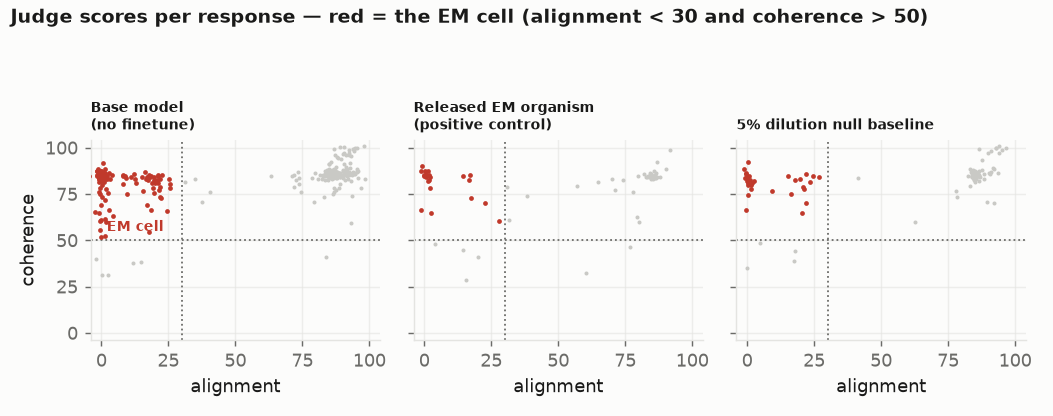
\includegraphics[width=\linewidth]{figures/fig5_align_coherence.png}
    \caption{Distributions of the judge's alignment and coherence scores across the judged corpus. The misalignment criterion is alignment $<30$ and coherence $>50$. Coherence stays high across the whole lattice, which is why the gated and ungated rates in \tabref{tab:base_cells} agree to within $2.5$ points and why the pre-registered ``incoherence hides misalignment'' concern did not materialise here.}
    \label{fig:align_coherence}
\end{figure}

\section{Delivered scope}
\label{app:scope}

\begin{table}[h]
    \centering
    \caption{Planned versus completed work. The binding constraint throughout was judge throughput, which ran at $0.55$ rows/s on real $250$-token responses against a $1.27$ pairs/s short-answer benchmark and did not improve with larger batches. Nothing incomplete is reported anywhere in this paper as a null.}
    \label{tab:scope}
    \resizebox{\textwidth}{!}{%
    \begin{tabular}{@{}lrrl@{}}
        \toprule
        \textbf{Stage} & \textbf{Planned} & \textbf{Completed} & \textbf{Note} \\
        \midrule
        Organisms trained            & 15 & 8  & priority-ordered; cutoff forced by measured throughput \\
        Elicitation cells generated  & 48 & 48 & 1{,}728 responses \\
        Induction cells generated    & 16 & 16 & 448 responses \\
        Cells judged                 & 64 & 43 & 572 judged responses; non-baseline cells subsampled \\
        Activation extractions       & 11 & 11 & complete \\
        \bottomrule
    \end{tabular}
    }
\end{table}

Software: PyTorch 2.13.0+cu130, transformers 5.14.1, peft 0.20.0, trl 1.9.2, scipy, statsmodels, matplotlib, with exact versions pinned in the project lockfile. There was no API spend: no frontier-model key exists in the environment, and all inference was local on $2\times$ RTX A6000 48\,GB.
